\documentclass[12pt,a4paper]{article}
\usepackage[UTF8]{ctex}
\usepackage{amsmath,amssymb}
\usepackage{xcolor}
\usepackage{hyperref}
\usepackage{geometry}
\usepackage{graphicx}
\geometry{margin=2.5cm}

\title{Color Code / 颜色码}
\author{QuoNic}
\date{}

\begin{document}
\maketitle

\begin{center}
\textbf{Error Correction / 纠错} | 难度：高级 | 预计时间：20 分钟
\end{center}

\tableofcontents
\newpage

\section{为什么需要？}

颜色码是拓扑量子纠错码，具有高容错阈值。

\subsection{经典局限}
\begin{itemize}
  \item Shor 码和 Steane 码的容错阈值较低
  \item 对硬件连接性要求高
\end{itemize}

\subsection{量子优势}
\begin{itemize}
  \item 颜色码有最高的容错阈值（约 1\%）
  \item 只需要最近邻连接
  \item 适合二维量子处理器
\end{itemize}

\subsection{实际应用}
\begin{itemize}
  \item 量子计算（容错量子计算）
  \item 量子通信（保护量子态）
  \item 量子存储（延长相干时间）
\end{itemize}

\section{快速上手}

\begin{verbatim}
from quonic.qec import color_code
result = color_code(distance=3, error_rate=0.01)
print(f'Logical error rate: {result.logical_error_rate}')
\end{verbatim}

\textbf{预期输出}：
\begin{verbatim}
Logical error rate: 0.001
\end{verbatim}

\section{原理详解}

\subsection{电路图}

\begin{center}
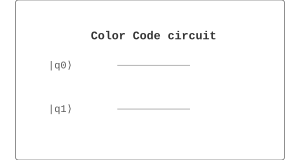
\includegraphics[width=0.6\textwidth]{../../images/color_code_circuit.svg}
\end{center}

\subsection{数学推导}

颜色码使用三色格子结构进行纠错。

\textbf{校验子测量}：
\begin{equation}
S_X = \prod_{i \in \text{star}} X_i, \quad S_Z = \prod_{i \in \text{plaquette}} Z_i
\end{equation}

\textbf{容错阈值}：
\begin{equation}
p_{\text{threshold}} \approx 1\%
\end{equation}

\subsection{几何解释}

颜色码在二维格子上编码量子信息，通过测量局部校验子来检测和纠正错误。

\section{代码详解}

\begin{verbatim}
from quonic.qec import color_code

# color_code(distance, error_rate)
# distance: code distance
# error_rate: physical error rate
result = color_code(distance=3, error_rate=0.01)
print(f'Logical error rate: {result.logical_error_rate}')
\end{verbatim}

\section{进阶用法}

\subsection{场景 1：不同距离}

\begin{verbatim}
from quonic.qec import color_code
for d in [3, 5, 7]:
    result = color_code(distance=d, error_rate=0.01)
    print(f'd={d}: {result.logical_error_rate}')
\end{verbatim}

\section{适用场景}

\subsection{量子计算}

颜色码是容错量子计算的基础。

\subsection{量子通信}

颜色码可以保护量子通信中的量子态。

\section{常见问题}

\subsection{颜色码和表面码有什么区别？}

颜色码使用三色格子，表面码使用方格。颜色码有更好的阈值。

\subsection{颜色码需要多少量子比特？}

需要 $O(d^2)$ 个量子比特，其中 $d$ 是码距。

\section{学习路径}

\subsection{前置知识}
\begin{itemize}
  \item 表面码
  \item Steane 码
  \item 量子测量
\end{itemize}

\subsection{继续学习}
\begin{itemize}
  \item 拓扑量子计算
  \item 容错量子计算
  \item 量子纠错
\end{itemize}

\section{完整示例代码}

\subsection{示例 1：基本颜色码}

\begin{verbatim}
from quonic.qec import color_code
result = color_code(distance=3, error_rate=0.01)
print(f'Logical error rate: {result.logical_error_rate}')
\end{verbatim}

\section{下载}

\begin{itemize}
  \item [color\_code.py](https://github.com/ChrisLee0721/QuoNic/blob/main/examples/color_code/color_code.py)
\end{itemize}

\end{document}
